
After being translated, a protein undergoes several processes before becoming mature. 5 important post-translational processes can be isolated (Figure \ref{fig:pTP}), even though they may occur in parallel. 3 processes are common to cytosolic, membrane and secreted proteins, namely
\begin{itemize}
\item Deformylation and demethylation.
\item Folding.
\item Residue modifications.
\end{itemize}

Moreover, there are 2 processes that specifically target membrane and secreted proteins
\begin{itemize}
\item Translocation.
\item Cleavage of the peptide signal and lipoprotein diacylglyceryl adduction.
\end{itemize}

\begin{figure}[!ht]
\centering
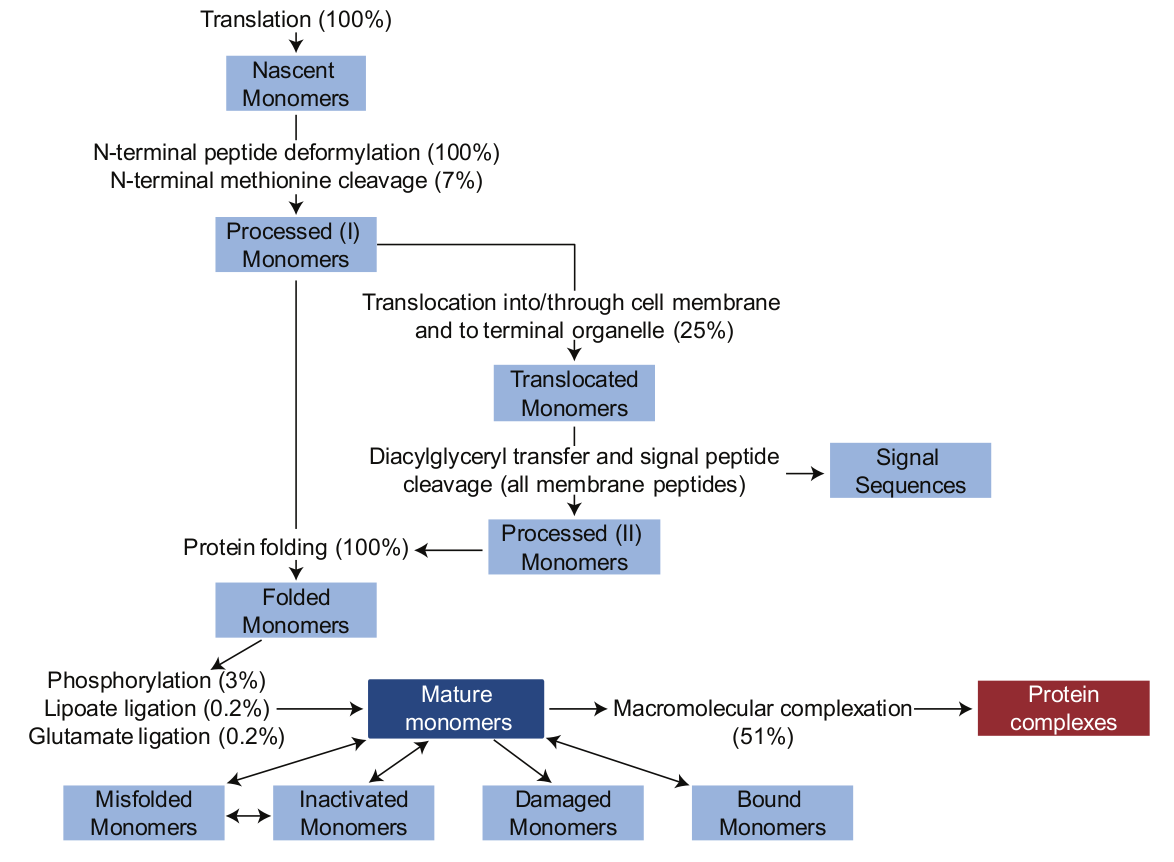
\includegraphics[width=0.8\linewidth]{figure/proteinProcesses}
\caption{Processes undergone by protein following translation (from Karr \textit{et al.})}
\label{fig:pTP}
\end{figure}

\subsubsection{Deformylation and demethylation}

For every protein, translation begins with a formylmethionine (fMet) residue. Several authors suggest that using exclusively fMet to start protein translation may be a way to regulate protein synthesis, as fMet is one of the most expensive amino acids to synthesize. Thus global protein synthesis levels would depend on global cell health.

This residue is then partially removed, but the role of deformylation and demethylation remains poorly understood. It may help in recycling fMet and influence protein degradation. According to the N-end rule, some N-terminal residues will lead to enhanced degradation. By changing the nature of the N-terminal residue, deformylation and demethylation allows for the N-end pathway to catalyze protein degradation.

Peptide deformylases (PDF) remove the formyl residue from fMet for most proteins. In \textit{B. subtilis}, YkrB is the main PDF, even though Def is known to have a similar action. It remains unclear whether these enzymes act during protein translation or after translation is completed. Methionine cleavage is performed by Methionine Aminopeptidases (MAP) but, contrarily to deformylation, it only targets a minority of proteins.

\subsubsection{Folding}

After translation, proteins can be viewed as a one-dimensional chain of amino acids. In order to acquire their functional form, proteins need to adopt a specific three-dimensional folding. Even though this folding is energetically favorable, numerous proteins need the help of another protein to adopt the proper conformation. These helper proteins are called chaperones. Bacteria use several chaperones. For example, in \textit{B. subtilis}
\begin{itemize}
\item The trigger factor Tig is known to assist early folding.
\item GroEL and its co-enzyme GroES assist late folding of short proteins.
\item DnaK, DnaJ and GrpE assist late folding of longer proteins.
\item FtsH may assist membrane protein folding.
\item Some proteins have specific chaperones (for example the translocated proteins TorA and NiFe are chaperoned by TorD and HybE respectively).
\end{itemize}

\subsubsection{Translocation, peptide signal cleavage and diacylglyceryl adduction}

During its life cycle, a bacterium heavily interacts with the extracellular medium. These interactions are enabled by proteins that are embedded in the membrane (nutrient transporters, ATP synthase, receptors, transducers) or secreted (virulence factors, cell wall components). Proteins that need to undergo translocation are identified by their N-terminal and C-terminal signal sequences (petide signals). Their embedding and secretion through the hydrophobic membrane is assisted by a specific machinery. 

Two important pathways are involved in protein translocation: Tat and SecA. They both involve a docking and a translocation step. Docking is mediated by peptide signals that can be recognized by signal recognition proteins (SRP) or directly by membrane proteins involved in the translocons (such as SecA or TatC). Translocation then occurs through a pore of variable size consisting of several proteins (SecYEG translocase or TatA like proteins). Depending on the nature of the proteins, translocation can occur simultaneously to translation (integral membrane proteins) or after translation (lipoproteins and secreted proteins). 

Following translocation, lipoproteins are anchored to the membrane through ligation of diacylglyceryl mediated by diacylglyceryl transferase and their peptide signal is removed by a signal peptidase. (what about the cleavage of peptide signals of secreted proteins and integral membrane proteins in \textit{B. subtilis} ???)


\subsubsection{Residue modifications}

Some proteins undergo post-translational chemical modifications. These modifications may serve different objectives such as favoring alternative conformations or regulating protein activity. Examples of residue modifications include phosphorylation, lipoyl transfer to lysine and $\alpha$-glutamate ligation, all catalyzed by specific enzymes.
